\documentclass[tikz,border=4pt]{standalone}
\usepackage[utf8]{inputenc}
\usepackage[T1]{fontenc}
\usepackage{helvet}
\renewcommand{\familydefault}{\sfdefault}
\usetikzlibrary{arrows.meta,positioning}
\begin{document}
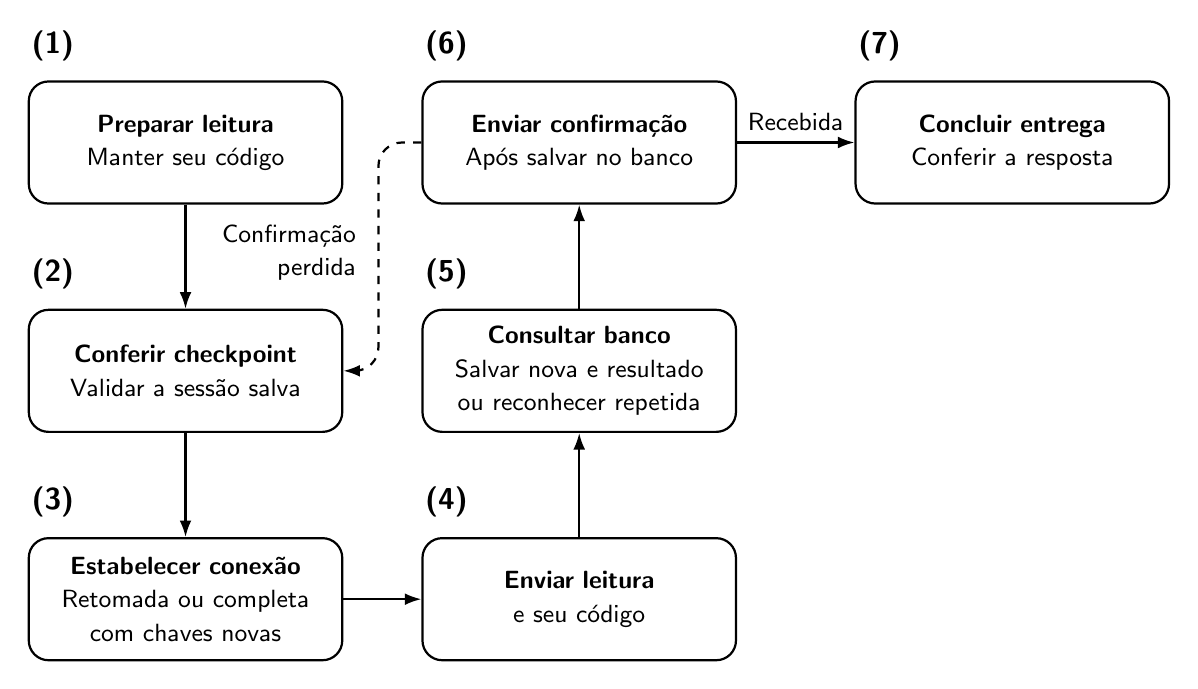
\begin{tikzpicture}[
  font=\sffamily\fontsize{9}{12}\selectfont,
  line width=0.8pt,
  flow/.style={-{Latex[length=2.1mm,width=1.5mm]},rounded corners=3mm},
  block/.style={draw=black,fill=white,rounded corners=2.5mm,
    text width=3.7cm,minimum height=1.55cm,align=center,inner sep=4pt},
  stage number/.style={font=\sffamily\bfseries\fontsize{11}{13}\selectfont,
    anchor=south west,inner sep=1pt},
  note/.style={font=\sffamily\fontsize{9}{12}\selectfont,
    align=left,inner sep=2pt}
]
\node[block] (reading) at (2,6)
  {\textbf{Preparar leitura}\\Manter seu código};
\node[block] (saved) at (2,3.1)
  {\textbf{Conferir checkpoint}\\Validar a sessão salva};
\node[block] (connect) at (2,0.2)
  {\textbf{Estabelecer conexão}\\Retomada ou completa\\com chaves novas};
\node[block] (send) at (7,0.2)
  {\textbf{Enviar leitura}\\e seu código};
\node[block] (process) at (7,3.1)
  {\textbf{Consultar banco}\\Salvar nova e resultado\\ou reconhecer repetida};
\node[block] (acknowledge) at (7,6)
  {\textbf{Enviar confirmação}\\Após salvar no banco};
\node[block] (finished) at (12.5,6)
  {\textbf{Concluir entrega}\\Conferir a resposta};

\foreach \n/\k in {reading/1,saved/2,connect/3,send/4,process/5,acknowledge/6,finished/7}
  \node[stage number] at ([yshift=2mm]\n.north west) {(\k)};

\draw[flow] (reading.south) -- (saved.north);
\draw[flow] (saved.south) -- (connect.north);
\draw[flow] (connect.east) -- (send.west);
\draw[flow] (send.north) -- (process.south);
\draw[flow] (process.north) -- (acknowledge.south);
\draw[flow] (acknowledge.east) --
  node[note,above=2pt] {Recebida} (finished.west);

% A confirmação perdida não gera outro identificador de leitura.
\draw[flow,dashed] (acknowledge.west) -- (4.45,6)
  -- (4.45,3.1) -- (saved.east);
\node[note,anchor=east,align=right] at (4.25,4.6)
  {Confirmação\\perdida};
\end{tikzpicture}
\end{document}
